\section{Analisi degli investimenti}
\subsection{Tasso di sconto}
Il tasso di sconto è stato calcolato utilizzando il modello CAPM - Capital Asset
Pricing Model, secondo cui il tasso di sconto è definito come
\begin{displaymath}
r = r_f + \beta (r_m - r_f )
\end{displaymath}
\begin{eqnarray*}
r_f &=& 0.0357 \qquad \mbox{tasso di rendimento di un titolo privo di rischi} \\ 
\beta &=& 1,24 \quad\qquad \mbox{fattore di rischio} \\
r_m &=& 0.0452 \qquad \mbox{tasso di rendimento medio del mercato}
\end{eqnarray*}

Da un’analisi del mercato italiano tecnologico abbiamo trovato come valori
$\beta=1,24$ e $r_m=4.52\%$. Come titolo risk-free è stato scelto il BTP
(\ref{finmer}), il cui tasso di rendimento a 5 anni è $r_f=3.57\%$ (data di
riferimento: 15/01/2019).\\ 
Il valore ottenuto è $r = 4.75\%$\\
Con tale tasso di sconto è possibile determinare dai flussi di cassa gli indici
VAN e TIR.
%
%
\subsection{Stima della domanda}
Si ipotizzata una domanda con crescita secondo una curva logistica del tipo: 
\begin{displaymath}
q(i) = \frac{1}{1 + \beta_1 e^{-i\beta_2}}
\end{displaymath}

Il numero di utenti potenziali è stato fissato ad $U=50.236$ (\ref{miele}).
Avendo ipotizzato una crescita con curva logistica, poniamo $q(1)=0.01$ e
$q(5)=0.05$ come proporzione di utenti interessati alla domanda nel periodo
interessato dalla nostra analisi.  

Si è ipotizzato ipotizzato inoltre che i clienti dispongano di una struttura che
racchiude il loro allevamento di api o che, in previsione dell’acquisto del
nostro prodotto, procedano con l’installazione di una struttura del genere. In
questo modo ogni cliente può acquistare un singolo prodotto da applicare
all’ingresso dell’allevamento evitando di acquistarne uno per ogni arnia.

Il numero di clienti che otteniamo anno per anno dalla domanda non è di tipo
cumulativo, questo perché un cliente che ha acquistato il prodotto non
è soggetto ad ulteriori spese negli anni successivi. Alla domanda di ogni periodo di
riferimento si è quindi sottratto i valori della domanda relativa ai periodi
precedenti, ottenendo il numero dei soli nuovi clienti interessati.

In un periodo di riferimento i flussi di cassa sono determinati dai ricavi
dovuti all’acquisto del prodotto da parte di nuovi clienti, pertanto la
proporzione di utenti che contribuiscono a tale calcolo viene calcolata come
$q(i) - q(i-1)$ per il periodo $i$ di riferimento. Questo spiega il calo di
domanda che c’è tra gli anni $t=1$ e $t=2$.

% tabella dcf
\begin{table}[!h]
%\centering
\begin{adjustbox}{width=\textwidth}
\begin{tabular}{c|c|r@{.}l|r@{.}l|r@{.}l|r@{.}l|c|r@{.}l}
& Nuovi 
& \multicolumn{2}{|c}{[\euro/utente]}
& \multicolumn{2}{|c}{[\euro]}
& \multicolumn{2}{|c}{[\euro]}
& \multicolumn{2}{|c|}{[\euro]}
& 
& \multicolumn{2}{|c}{[\euro]}
\\
Anno
& Utenti
& \multicolumn{2}{|c}{OPEX}
& \multicolumn{2}{|c}{Ricavi Netti}
& \multicolumn{2}{|c}{CAPEX}
& \multicolumn{2}{|c|}{CF}
& $(1+r)^{-i}$
& \multicolumn{2}{|c}{DCF}
\\

\hline
0 &      &   0&00 &      0&00 & -5080&00&  -5080&00 &1.00& -5080&00 \\
1 & 502  & 266&61 &  41861&78 &     0&00&  41861&78 &0.92& 38512&84 \\ 
2 & 253  & 386&01 &  -9110&53 &     0&00&  -9110&53 &0.84& -7652&85 \\
3 & 377  & 306&84 &  16271&32 &     0&00&  16271&32 &0.77& 12528&92 \\
4 & 558  & 254&43 &  53322&48 &     0&00&  53322&48 &0.71& 37858&96 \\
5 & 820  & 219&57 & 106952&60 &     0&00& 106952&6  &0.65& 69519&19
\end{tabular}
\end{adjustbox}
\caption{Flussi di cassa scontati}
\label{tab:dcf}
\end{table}

 





%
\begin{figure}[!h]
\centering
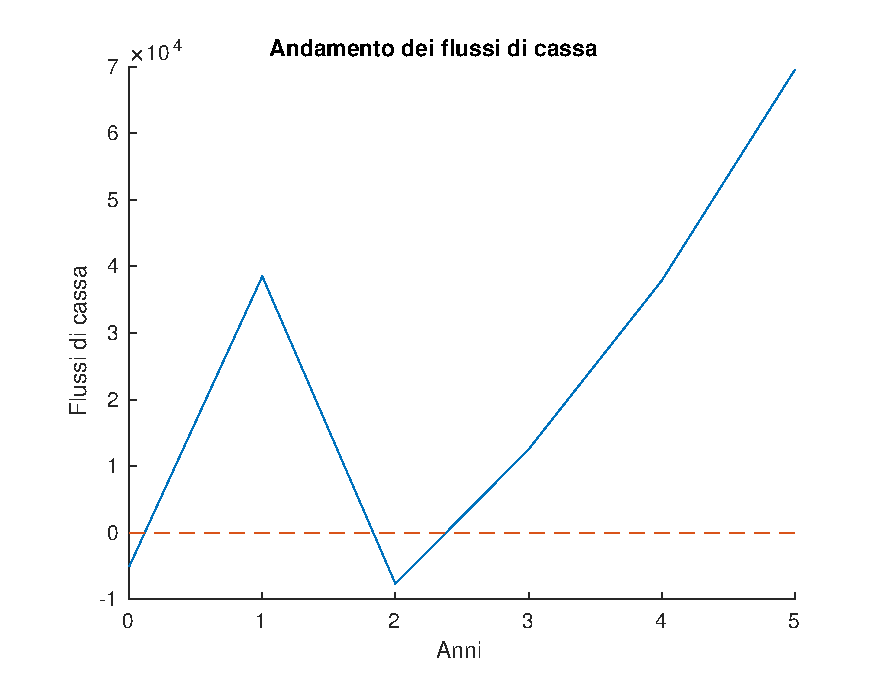
\includegraphics[width=\textwidth]{figures/cf}
\caption{Flussi di cassa scontati relativi primi 5 anni di attività}
\label{cf}
\end{figure}
%
%%%%%%%%%%%%%%%%%%%%%%%%%%%%%%%%%%%%%%%%%%%%%%%%%%%%%%%%%%%%%%%%%%%%%%%%%%%%%%%%
%%%%%%%%%%%%%%%%%%%%%%%%%%%%%%%%%%%%%%%%%%%%%%%%%%%%%%%%%%%%%%%%%%%%%%%%%%%%%%%%
%%%%%%%%%%%%%%%%%%%%%%%%%%%%%%%%%%%%%%%%%%%%%%%%%%%%%%%%%%%%%%%%%%%%%%%%%%%%%%%%
\subsection{VAN e TIR}
I flussi di cassa (guadagno netto - costi ricorrenti) dall’anno $t=0$ a $t=5$ sono
rappresentati nella tabella~\ref{tab:van} insieme al VAN cumulativo.
Il VAN è calcolato come 	
\begin{displaymath}
VAN = - C_0 + \sum_{i=1}^n \frac{F_i}{(1 + r)^i}
\end{displaymath}
\begin{eqnarray*}
C_0 &=& 80000 \ \mbox{\euro} \qquad \mbox{investimento iniziale} \\
r &=& 0.0475 \qquad \mbox{tasso di sconto} \\
n &:=& \mbox{numero di periodi analizzati} \\
F_i &:=& \mbox{flusso di cassa relativo al periodo i}
\end{eqnarray*}
% tabella van
\begin{table}[!h]
\centering
%\begin{adjustbox}{width=\textwidth}
\begin{tabular}{c|r@{.}l|r@{.}l}
Anno
& \multicolumn{2}{|c}{$F_i$ [\euro]}
& \multicolumn{2}{|c}{VAN [\euro]}
\\          
\hline
0 & -5080&00 & -85080&00 \\
1 & 38512&84 & -46567&16 \\ 
2 & -7652&85 & -54220&01 \\
3 & 12528&92 & -41691&09 \\
4 & 37858&96 &  -3832&13 \\
5 & 69519&19 &  \textbf{65687}&\textbf{06} 
\end{tabular}
%\end{adjustbox}
\caption{Valore Attuale Netto}
\label{tab:van}
\end{table}

%
\begin{figure}[!h]
\centering
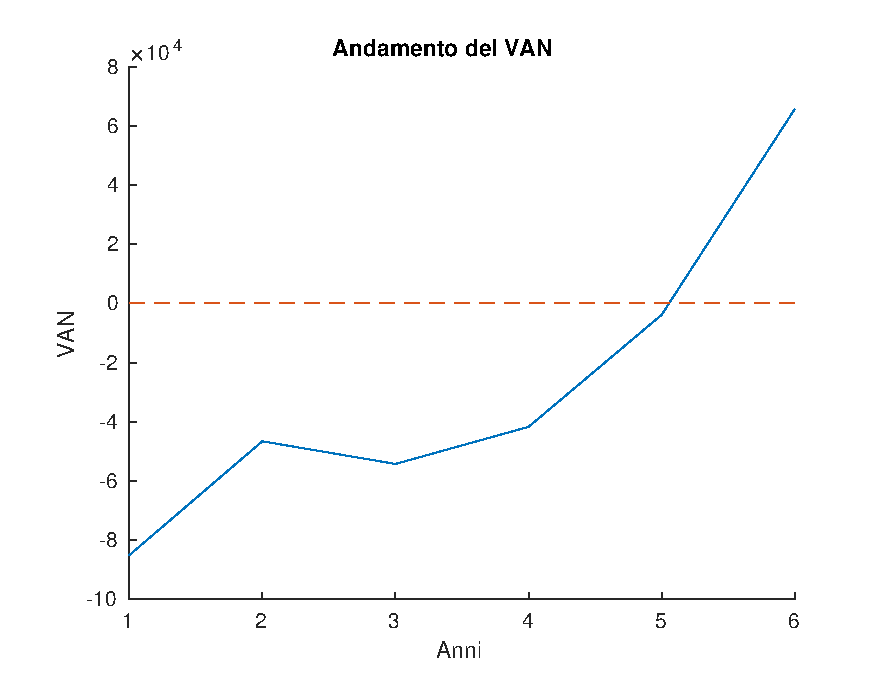
\includegraphics[width=\textwidth]{figures/van}
\caption{Andamento del VAN nei primi 5 anni di attività}
\label{van}
\end{figure}
%
Il periodo di pareggio finanziario (“payback period”) è dunque raggiunto tra il
quarto ed il quinto anno. Essendo un indice che può essere interpretato come
grado di rischio associato al progetto, ci si può ritenere soddisfatti di poter
mostrare che entro il quinto anno di esercizio la nostra azienda può raggiungere
il pareggio e ottenere un VAN positivo. L'andamento del VAN durante i primi 5
anni è mostrato in figura~\ref{van}.

Il TIR è il tasso di attualizzazione per cui il VAN del progetto è pari a zero, 
ed è usato per misurare la redditività di progetti e investimenti.
Studiando il valore del VAN al variare del tasso di sconto, e riducendo
l’intervallo ricercando di volta in volta il valore del VAN nel punto medio,
si è giunti all’intervallo \mbox{$[8.50, 8.51]$}. Il valore del VAN agli estremi è
$VAN(r = 8.50) = 651.29 \mbox{\euro}$ e $VAN(r=8.51) = -139.68 \mbox{\euro}$,
dunque scegliendo il punto intermedio si ottiene $TIR = 8.505\%$.
%%%%%%%%%%%%%%%%%%%%%%%%%%%%%%%%%%%%%%%%%%%%%%%%%%%%%%%%%%%%%%%%%%%%%%%%%%%%%%%%
%%%%%%%%%%%%%%%%%%%%%%%%%%%%%%%%%%%%%%%%%%%%%%%%%%%%%%%%%%%%%%%%%%%%%%%%%%%%%%%%
%%%%%%%%%%%%%%%%%%%%%%%%%%%%%%%%%%%%%%%%%%%%%%%%%%%%%%%%%%%%%%%%%%%%%%%%%%%%%%%%
\subsection{Valutazione del rischio}
I rischi individuati per il prodotto in relazione alla loro natura sono:
\begin{itemize}
\item Rischi puri: incendi, terremoti, guasti nelle attrezzature;
\item Rischi speculativi: oscillazione dei tassi di cambio, innovazioni
tecnologiche (per esempio rappresentate dall’utilizzo di droni), variazioni nel
costo dell’hardware, variazione di costi operativi.
\end{itemize}

Sono stati valutati una serie di rischi significativi, analizzando singolarmente
l’incidenza sull’andamento del VAN. Non abbiamo tenuto conto del rischio di
incendi in quanto molto basso in percentuale nel nostro caso, visto che la
probabilità di incendio viene calcolata in base diretta al numero di dipendenti,
la grandezza dell’immobile e la quantità di materiale infiammabile. Il rischio
per terremoti non è stato considerato in quanto, ipotizzando di avere la nostra
società a Roma, siamo in un’area con bassa probabilità di attività sismica.

Per osservare l’incidenza di ogni fattore di rischio si fissata una
percentuale di variazione dei parametri associati pari al 10\%. Si è quindi
calcolato il VAN sia nel caso in cui tale variazione sia positiva che negativa,
e si è determinata la sua variazione percentuale rispetto al VAN ottenuto nel
caso “reale”.

I risultati sono rappresentati nel “diagramma tornado” in figura~\ref{tornado} e
nella tabella~\ref{tab:risk}, che mostrano i fattori di rischio ordinati in base
alla loro incidenza sul VAN.
\begin{table}[!h]
\centering
%\begin{adjustbox}{width=\textwidth}
\begin{tabular}{c|c|c|r@{.}l|r@{.}l}
& Valore 
&
& \multicolumn{2}{|c}{}
& \multicolumn{2}{|c}{Percentuale}
\\
Parametro
& attuale
& Variazione 
& \multicolumn{2}{|c}{VAN [\euro]}
& \multicolumn{2}{|c}{variazione}
\\

\hline
Domanda    &            &                          & 50780&78 & 271&67\%  \\
           &            &                          &-23456&60 &-271&68\%  \\
\hline                                  
Costo      & \EUR{1000} & $ + 100 \ \mbox{\euro} $ &  8441&81 & -38&21\%  \\
affitto    &            & $ - 100 \ \mbox{\euro} $ & 18885&13 & +38&22\%  \\
\hline                  
Costo      & \EUR{115}  & $+ 11.5 \ \mbox{\euro} $ & 38342&71 & 180&63\%  \\
hardware   &            & $- 11.5 \ \mbox{\euro} $ &-11016&67 &-180&63\%  \\
\end{tabular}
%\end{adjustbox}
\caption{Variazione del VAN al variare dei parametri coinvolti dai rischi}
\label{tab:risk}
\end{table}

%
\begin{figure}[!h]
\centering
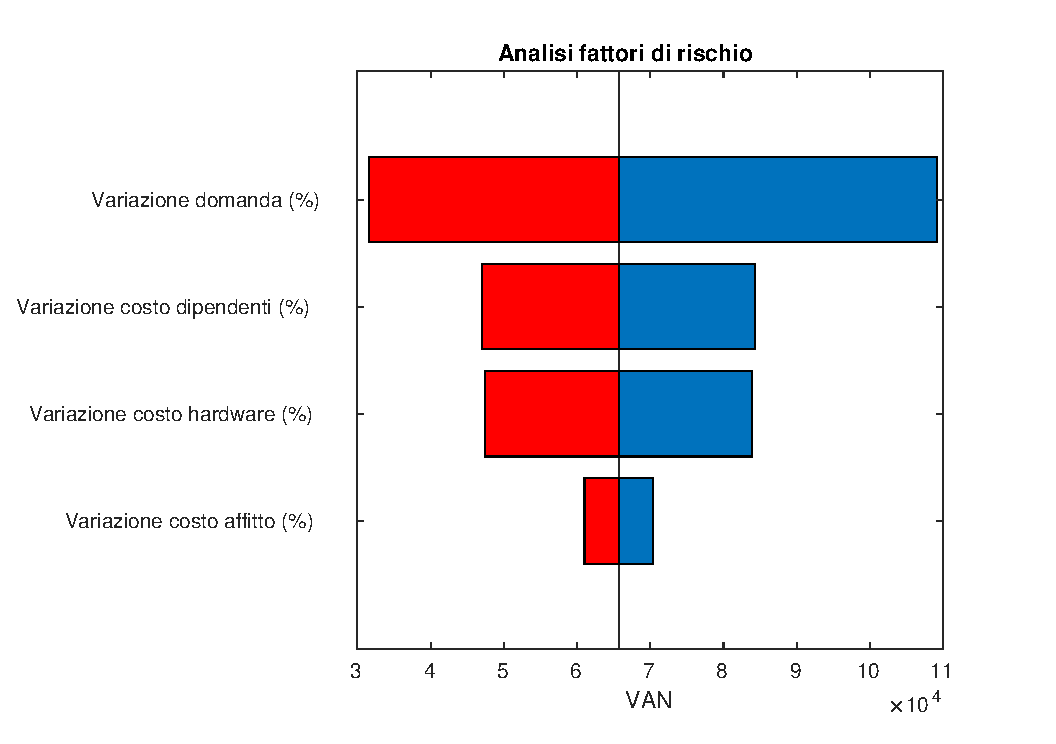
\includegraphics[width=\textwidth]{figures/tornado}
\caption{Diagramma tornado associato ai rischi}
\label{tornado}
\end{figure}
%
Il fattore di rischio con incidenza maggiore è rappresentato dal “fattore
di markup”. La “domanda” e il “costo dell’hardware” hanno un’incidenza media,
mentre i “costi relativi all’affitto” e il “tasso di sconto” hanno un’incidenza
minore.
%%%%%%%%%%%%%%%%%%%%%%%%%%%%%%%%%%%%%%%%%%%%%%%%%%%%%%%%%%%%%%%%%%%%%%%%%%%%%%%%
%%%%%%%%%%%%%%%%%%%%%%%%%%%%%%%%%%%%%%%%%%%%%%%%%%%%%%%%%%%%%%%%%%%%%%%%%%%%%%%%
%%%%%%%%%%%%%%%%%%%%%%%%%%%%%%%%%%%%%%%%%%%%%%%%%%%%%%%%%%%%%%%%%%%%%%%%%%%%%%%%
\subsection{Modello WACC}
Per analizzare le fonti di finanziamento del nostro prodotto è stato utilizzato
il Modello WACC - Weighted Average Cost of Capital, il quale restituisce il
costo medio ponderato del capitale.
\begin{displaymath}
WACC = k_D \frac{D}{D+E} + k_E \frac{E}{D+E}
\end{displaymath}
\begin{eqnarray*}
k_D &=& 0.0475 \quad \mbox{costo del debito al netto della fiscalità} \\
k_E &=& 0.0650 \quad \mbox{costo del capitale proprio. E’ il tasso di sconto “r”} \\
D &=& 0.5 \quad \mbox{valore del debito gravato da interessi} \\
E &=& 0.5 \quad \mbox{valore del patrimonio netto} 
\end{eqnarray*}
Si è ipotizzato di avere il 50\% delle fonti di finanziamento rappresentati da
capitale proprio, e il restante 50\% da un finanziamento. Quindi $\frac{D}{D+E} 
= \frac{E}{D+E} = 0.5$.  $k_E$ come già calcolato è pari a 4.75\%, mentre per il
costo del debito visto l’elevato rischio di una azienda “neonata” al primo anno
di attività si è imposto $k_D = 6.5\%$. 

Si ottiene un WACC = 0.056 e dal confronto con il TIR si può valutare se è
conveniente investire o meno nel nostro progetto. Poiché $TIR = 0.08505 > 0.056$
si può concludere che è conveniente.
